%% Article for Hyperfine Interactions (Springer)
%% Uses svjour3.cls — compile from docs/ where svjour3.cls lives.
%% Compile with: pdflatex → bibtex → pdflatex → pdflatex

\documentclass[smallcondensed]{svjour3}
\smartqed

\usepackage[T1]{fontenc}
\usepackage[utf8]{inputenc}
\usepackage{graphicx}
\usepackage{amsmath,amssymb}
\usepackage{booktabs}
\usepackage{siunitx}
\usepackage{svg}            % \includesvg — requires Inkscape on PATH
\usepackage{xcolor}
\usepackage{multirow}
\usepackage{url}
\usepackage{doi}

\sisetup{
  separate-uncertainty = true,
  range-phrase = --,
}

\journalname{Interactions}  % Renamed from Hyperfine Interactions in 2024

% ─────────────────────────────────────────────────────────────────────────────
\begin{document}

\title{Fitbauer: an open-source Python application for
       $^{57}$Fe M\"{o}ssbauer spectral analysis
       with rigorous uncertainty quantification}

\titlerunning{Fitbauer: open-source $^{57}$Fe M\"{o}ssbauer fitting}

\author{Jorge S\'anchez Marcos \and
        Nieves Men\'endez Gonz\'alez}

\authorrunning{S\'anchez Marcos \& Men\'endez Gonz\'alez}

\institute{J.~S\'anchez Marcos \and N.~Men\'endez Gonz\'alez \at
           Departamento de Qu\'imica F\'isica, Facultad de Ciencias,
           Universidad Aut\'onoma de Madrid,
           Campus de Cantoblanco, 28049 Madrid, Spain \\
           \email{jorge.sanchezm@uam.es}}

\date{Received: \today}

\maketitle

% ─────────────────────────────────────────────────────────────────────────────
\begin{abstract}
We present \textbf{Fitbauer}, an open-source desktop application
written in Python for the analysis, simulation, and least-squares fitting
of $^{57}$Fe M\"{o}ssbauer transmission spectra.
The program is built around \emph{live simulation} of the direct model:
every parameter change re-renders the spectrum instantly, so a physically
sensible model can be constructed by eye before fitting.
It implements discrete fitting of up to six simultaneous components
(singlets, doublets, sextets, and magnetic-relaxation lineshapes),
as well as hyperfine field distributions $P(B_\mathrm{hf})$
and quadrupole-splitting distributions $P(\Delta E_Q)$ with Tikhonov,
total-variation, or maximum-entropy regularisation
(Hesse--R\"{u}bartsch method).
Three independent uncertainty-quantification methods are provided:
propagated covariance matrices, residual bootstrap Monte Carlo,
and profile-likelihood intervals.
A rigorous validation suite comprising 34 automated tests at six levels ---
from mathematical self-consistency to Monte Carlo pull statistics ---
is included in the distribution.
A direct comparison with NORMOS/SITE (Brand 1987) on identical spectra
of $\alpha$-Fe, hematite ($\alpha$-Fe$_2$O$_3$), siderite (FeCO$_3$),
and magnetite (Fe$_3$O$_4$) shows agreement in all hyperfine parameters
to within \SI{0.013}{\tesla} in $B_\mathrm{hf}$ and
\SI{0.004}{\milli\metre\per\second} in $\delta$,
confirming the correctness of the physical model and calibration.
The program is platform-independent (Windows, Linux, macOS),
offers an interface in seven languages,
and is freely available under an open licence.

\keywords{M\"{o}ssbauer spectroscopy \and Spectral fitting \and
          Hyperfine parameters \and Distribution analysis \and
          Open source \and Python \and Uncertainty quantification}
\end{abstract}

% ─────────────────────────────────────────────────────────────────────────────
\section{Introduction}
\label{sec:intro}

$^{57}$Fe M\"{o}ssbauer spectroscopy remains one of the most direct
probes of local electronic structure, magnetic order, and oxidation
state in iron-containing compounds. Its widespread use in mineralogy,
environmental science, materials science, and geochemistry depends
critically on the quality of spectral fitting software used to extract
hyperfine parameters from the data~\cite{Greenwood1971,Gütlich2011}.

Several programs have been developed over the past four decades.
NORMOS~\cite{Brand1987} and its Windows wrapper WinNormos are the
most widely cited; they are written in Fortran and have served the
community well but are no longer actively developed and lack modern
graphical interfaces.
MossWinn~\cite{Klencsar2013} (Z.~Klencsar, Budapest) is a comprehensive
commercial package for Windows only, with outstanding features for
thick-absorber correction and a large spectral database.
SpectrRelax~\cite{Matsnev2012} handles relaxation and distribution
models on Windows. Moessfit~\cite{Kamusella2016} is a free Qt/C++
program focused on simultaneous multi-dataset fitting and the Maximum
Entropy Method. RECOIL~\cite{Lagarec1998} (University of Ottawa) and
VINDA~\cite{vinda} are further established options, likewise platform-restricted.
None of these programs is open source, which limits reproducibility
and makes independent code auditing impossible.

Recent years have seen growing demand for Python-based scientific software
owing to its ecosystem of well-tested numerical libraries, its suitability
for integration into automated pipelines, and the reproducibility of
virtual-environment setups~\cite{Virtanen2020}.
Here we describe Fitbauer, which was designed from the outset with three
goals: (i) full separation of the physics engine from any graphical interface,
enabling headless (scriptable/CLI) operation; (ii) a comprehensive and
formally validated uncertainty-quantification framework; (iii) a modern,
cross-platform interface built around \emph{live simulation} of the direct
model, available in seven languages.

Section~\ref{sec:model} describes the physical model.
Section~\ref{sec:arch} outlines the software architecture.
Section~\ref{sec:features} summarises the main features.
Section~\ref{sec:validation} presents the validation suite.
Section~\ref{sec:examples} shows application to four reference materials
including a direct comparison with NORMOS.
Section~\ref{sec:discussion} discusses advantages and current limitations.
Section~\ref{sec:conclusions} concludes.

% ─────────────────────────────────────────────────────────────────────────────
\section{Physical model}
\label{sec:model}

\subsection{Lineshape and transmission}

Fitbauer evaluates the M\"{o}ssbauer transmission spectrum in the
\emph{thin-absorber} approximation as:
\begin{equation}
  T(v) = B + sv
        - \sum_{k=1}^{N} A_k(v) ,
  \label{eq:model}
\end{equation}
where $B$ is the baseline (normalised), $s$ is an optional linear slope
accounting for slow background drift, $v$ is the source velocity, and
$A_k(v)$ is the absorption contribution of the $k$-th component.

Each Lorentzian line has the form
\begin{equation}
  L(v;\, v_0,\Gamma) = \frac{(\Gamma/2)^2}{(v-v_0)^2 + (\Gamma/2)^2} ,
\end{equation}
where $v_0$ is the line centre and $\Gamma$ is the full width at half
maximum (FWHM). A Voigt profile (convolution with a Gaussian of width
$\sigma$) is also available, evaluated via the Faddeeva function
(\texttt{scipy.special.wofz}) and normalised to its peak analytically,
independently of the velocity sampling.

Spectra recorded with a triangular velocity drive are folded around an
automatically refined folding point; sinusoidal-drive data
(NORMOS convention \texttt{TRIANG=.FALSE.}) are handled unfolded, with
each channel evaluated at its true sinusoidal velocity and the drive
phase available as a free fit parameter.

\subsection{Discrete components}
\label{sec:discrete}

Up to six spectral components can be superimposed; each is one of six
types: singlet, doublet, sextet, or one of three magnetic-relaxation
lineshapes (Section~\ref{sec:relax}).

\subsubsection{Sextet and quadrupole treatment}

For a sextet the conventional first-order correction applies
$\pm\Delta E_Q/2$ (inner/outer pairs). When $\Delta E_Q$ is large, an
exact Kündig diagonalisation~\cite{Kuendig1967} of the excited-state
Hamiltonian
\begin{equation}
  \hat{H} = \omega_L \hat{I}_z
  + \frac{\Delta E_Q}{6}
    \bigl(3\hat{I}_{z'}^2 - \hat{I}(\hat{I}+1)\bigr)
  \label{eq:kuendig}
\end{equation}
is available in fixed-angle or powder-average (\mbox{20-point}
Gauss--Legendre) variants. Line intensities follow the $3:2:1$ pattern
or are parameterised by the texture angle $t = \langle\sin^2\theta\rangle$.

\subsubsection{Thick-absorber correction}

For optically thick samples the transmission is modelled
as~\cite{Margulies1961}
\begin{equation}
  T(v) = b + sv - C\bigl(1 - e^{-A_\mathrm{tot}(v)/C}\bigr),
\end{equation}
where $b$ and $s$ are the baseline and slope, $A_\mathrm{tot}$ is the
thin-absorber absorption, and $C$ is the saturation scale.

\subsection{Magnetic relaxation models}
\label{sec:relax}

Although the main focus of the program is crystalline (discrete) fitting,
three relaxation lineshapes can be combined freely with discrete phases:
a phenomenological interpolation between a blocked sextet and a
superparamagnetic doublet; a two-state dynamic model for the
$+B_\mathrm{hf} \leftrightarrow -B_\mathrm{hf}$ exchange following
Blume and Tjon~\cite{BluemeTjon1968}; and a N\'{e}el--Arrhenius
model~\cite{Neel1949,Brown1963} for polydisperse nanoparticle assemblies
(lognormal size distribution, with an optional multi-temperature global
fit that shares the physical parameters across spectra).

\subsection{Hyperfine field and quadrupole-splitting distributions}
\label{sec:dist}

For magnetically disordered or nanostructured samples,
Fitbauer implements $P(B_\mathrm{hf})$ and $P(\Delta E_Q)$
distributions following the Hesse--R\"{u}bartsch
method~\cite{Hesse1974}: a sum of many sextets (or doublets)
on a uniform grid, with amplitudes constrained to be non-negative
and regularised by minimising
\begin{equation}
  F = \|\mathbf{y} - \mathbf{A}\mathbf{p}\|_w^2
    + \alpha\,\|\mathbf{D}^2\mathbf{p}\|^2, \quad \mathbf{p}\geq 0 ,
  \label{eq:tikhonov}
\end{equation}
where $\|\cdot\|_w$ is the Poisson-weighted norm and $\mathbf{D}^2$ is
the second-difference matrix. Besides the Tikhonov penalty of
Eq.~\eqref{eq:tikhonov}, total-variation (edge-preserving) and
maximum-entropy regularisers are available.
The regularisation parameter $\alpha$ is selected via the L-curve
criterion~\cite{Hansen1992} --- with suggestions from maximum curvature,
a compromise value, and Generalised Cross-Validation (GCV) --- and can be
chosen interactively by clicking directly on the L-curve plot.
A $1\sigma$ uncertainty band on $P$ is computed from the linearised
covariance of the weights, and $\tilde{\chi}^2$ uses effective
degrees of freedom (trace of the hat matrix).
Simultaneous \emph{sharp} (discrete) components can be superimposed
on the distribution to handle multiphase samples.

As an alternative to the free-form histogram, parametric shapes can be
fitted without any regularisation: a single Gaussian, a binomial (alloy)
distribution, and the Voigt-based sum-of-Gaussians of Rancourt and
Ping~\cite{Rancourt1991}, in which the fitted amplitude of each Gaussian
directly gives the \emph{area} (population) of the corresponding
subpopulation.
Two-dimensional distributions such as $P(B_\mathrm{hf},\Delta E_Q)$ are
also available, with independent regularisation parameters in each
direction.

\subsection{Calibration convention}
\label{sec:calib}

The velocity calibration follows the standard $\alpha$-Fe convention:
$B_\mathrm{hf} \equiv \SI{33.0}{\tesla}$ with line positions
from published experimental measurements~\cite{Kalvius1969}
(\SI{\pm 0.839}{}$/$\SI{\pm 3.084}{}$/$\SI{\pm 5.329}{\milli\metre\per\second}),
not from nuclear moments.
Using theoretical positions introduces a systematic error of
$\approx\SI{0.1}{\tesla}$ in all fitted fields~\cite{FitbauerChangelog}.
Once determined from an $\alpha$-Fe foil, the calibration is \emph{fixed}
and reused automatically for every subsequent raw-counts spectrum, so the
velocity scale is defined once per instrument configuration.

% ─────────────────────────────────────────────────────────────────────────────
\section{Software architecture}
\label{sec:arch}

Fitbauer follows a strict Model--View--Controller separation.
The physics and optimisation code lives entirely in the \texttt{core/}
package, with no dependency on any graphical toolkit.
The Qt front-end (\texttt{PySide6}) and the command-line interface
are thin clients of \texttt{core/}.
This design allows the same computation to be driven interactively,
from a Python script, or from a batch pipeline without modification.

\begin{description}
  \item[\texttt{core/physics.py}] Pure functions for lineshape evaluation
    (Lorentzian, Voigt, thick-absorber), component absorption,
    and the Kündig Hamiltonian.

  \item[\texttt{core/fit\_engine.py}] Least-squares optimisation
    via \texttt{scipy.optimize.least\_squares} (bounded
    trust-region-reflective), multi-start initialisation,
    parameter bounds, covariance-matrix uncertainties,
    bootstrap resampling, and profile-likelihood intervals.

  \item[\texttt{core/folding.py}] Spectrum loading (WS5 XML and
    single-column ASCII ADT formats), automatic folding-point search,
    triangular- and sinusoidal-drive velocity axes.

  \item[\texttt{core/session.py}] Headless orchestration layer
    (\texttt{HeadlessSession}, \texttt{ModelState}):
    load $\to$ fold $\to$ fit $\to$ export without any GUI.

  \item[\texttt{mossbauer\_distribution.py}] Distribution fitting
    $P(B_\mathrm{hf})$/$P(\Delta E_Q)$: Tikhonov regularisation,
    L-curve, and sharp components.
\end{description}

Figs.~\ref{fig:gui-main} and \ref{fig:gui-fit} show the main graphical interface
and a discrete-fit result.

\begin{figure*}[t]
  \centering
  
\includegraphics[width=\textwidth]{img/captura-pantalla-principal}
  \caption{Fitbauer main window showing a fitted $\alpha$-Fe calibration
           spectrum (folded, $^{57}$Co/Rh source).
           Left: file status, calibration, folding, and background controls.
           Centre: Matplotlib plot area with data, model, and residuals.
           Right: simulation/fit panel with the physical parameters of the
           active component (here a sextet with $B_\mathrm{hf}$ fixed at
           \SI{33}{\tesla} while the velocity scale is fitted).}
  \label{fig:gui-main}
\end{figure*}

\begin{figure*}[t]
  \centering
  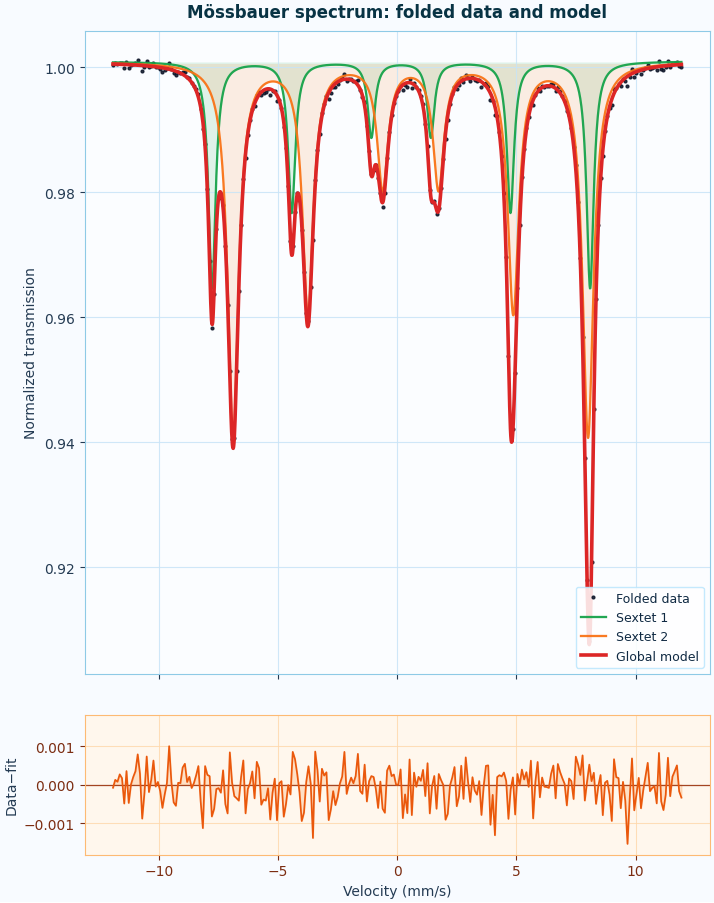
\includegraphics[width=\textwidth]{img/captura-ajuste-discreto}
  \caption{Discrete fitting of a two-component spectrum (magnetite Fe$_3$O$_4$).
           The two sextet subspectra are shown individually in colour with
           optional area shading; the total model is the thick red curve;
           residuals in the lower panel.}
  \label{fig:gui-fit}
\end{figure*}

% ─────────────────────────────────────────────────────────────────────────────
\section{Main features}
\label{sec:features}

\subsection{Live simulation of the direct model}
\label{sec:simulation}

A distinguishing design choice is that the direct model is always
\emph{live}: every slider or numeric change to any physical parameter
($\delta$, $\Delta E_Q$, $B_\mathrm{hf}$, widths, depths, intensities)
re-renders the full spectrum and its individual subspectra instantly.
This serves several practical purposes:
(i) a physically sensible starting model can be constructed by eye
before launching the optimiser, which makes the subsequent non-linear
fit faster and far less likely to fall into a spurious minimum;
(ii) the effect of each hyperfine parameter on the lineshape can be
explored interactively, which builds physical intuition and makes the
program useful for teaching;
(iii) hypotheses can be compared visually --- e.g.\ simulating a
two-phase mixture with assumed proportions over a measured spectrum ---
without fitting anything.
Simulation and fitting share exactly the same direct model, so what is
simulated is precisely what the optimiser will refine; per-parameter
\emph{fix} locks let the user freeze any subset of parameters during
this exploration and during the fit.

\subsection{Fitting modes}

\emph{Discrete mode} supports up to six simultaneous components
of any type, with independent free/fixed flags for each parameter,
linear constraints between parameters, and multi-start optimisation
(eight Gaussian restarts around the user's starting point with early
stopping, plus an optional differential-evolution pre-pass for
multi-sextet label-permutation minima).
The noise model can be Gaussian or Poissonian (iteratively reweighted
least squares with model-based variances).

\emph{Distribution mode} (Fig.~\ref{fig:gui-dist}) computes
$P(B_\mathrm{hf})$ or $P(\Delta E_Q)$ over a user-defined grid,
optionally with simultaneously fitted sharp components.
The regularisation parameter is selected interactively via the
L-curve (Fig.~\ref{fig:gui-lcurve}) or set manually.

\begin{figure}[t]
  \centering
  
\includegraphics[width=\columnwidth]{img/captura-distribucion-bhf}
  \caption{Distribution fitting of a magnetically disordered sample
           (synthetic spectrum generated from a bimodal
           $P(B_\mathrm{hf})$ at 28 and \SI{48}{\tesla}).
           Left: fitted spectrum and residuals.
           Right: reconstructed $P(B_\mathrm{hf})$, which recovers the
           two field populations.}
  \label{fig:gui-dist}
\end{figure}

\begin{figure}[t]
  \centering
  
\includegraphics[width=\columnwidth]{img/captura-lcurve}
  \caption{L-curve tool for regularisation-parameter selection.
           Left: $\|\mathbf{r}\|$ vs.\ $\|\mathbf{L}\cdot\mathbf{P}\|$
           with the automatically detected corner;
           right: RMS residual as a function of $\alpha$.
           Clicking on either panel selects the nearest scanned $\alpha$,
           so the automatic suggestion can be overridden by eye.}
  \label{fig:gui-lcurve}
\end{figure}

\subsection{Uncertainty quantification}

Three methods are provided and can be run consecutively on the
same fit:

\begin{enumerate}
  \item \emph{Covariance matrix} (default): symmetric $1\sigma$ errors
    from the Jacobian at the minimum,
    $\sigma_i = \sqrt{(J^\top J)^{-1}_{ii}}$.

  \item \emph{Bootstrap Monte Carlo}: $N$ replicas are generated
    by adding Poissonian noise at the per-channel level;
    each replica is independently refitted and the distribution
    of the $N$ best-fit values gives asymmetric percentile intervals.

  \item \emph{Profile likelihood}: the parameter of interest is
    stepped away from its best-fit value while all others are
    re-optimised; the $1\sigma$ interval corresponds to a unit
    increase in $\tilde{\chi}^2$~\cite{Rolke2005}.
\end{enumerate}

\subsection{Other features}

Further tools include batch fitting of spectrum series with warm-start
from the previous result, a semi-manual absorption-minima editor that
proposes starting models from the detected line positions,
PDF/Markdown report export, and reproducible session files that store
the complete analysis state (data, calibration, model, and results).
The interface is available in seven languages
(Spanish, English, French, German, Japanese, Russian, and Chinese).

% ─────────────────────────────────────────────────────────────────────────────
\section{Validation suite}
\label{sec:validation}

The distribution includes \texttt{tests/test\_synthetic\_validation.py},
a 34-test module structured in six levels of increasing rigour
(part of a wider automated suite covering the physics core, folding,
fit engine, distributions, and the graphical interface).

\subsection{Level 1 — Self-consistency}

Noise-free synthetic spectra are generated with a reference
implementation that is \emph{mathematically independent} of
\texttt{core/physics.py} (different variable names, no shared code),
and then fitted with Fitbauer.
The expected result is $\tilde{\chi}^2 < 10^{-6}$ and recovered
parameters identical to the ground truth to machine precision.
This level catches model bugs that would be invisible when testing
only with experimental data.

\subsection{Level 2 — Jacobian}

The analytical Jacobian of the model with respect to each free
parameter is compared against the finite-difference approximation
from \texttt{scipy.optimize.approx\_fprime}.
Maximum allowed relative discrepancy: 1\,\%.
Five independent checks cover singlet, doublet, sextet,
multi-component, and thick-absorber cases.

\subsection{Level 3 — Monte Carlo pull statistics}

$N=200$ synthetic spectra are drawn for each component type
with Poissonian noise at \num{8000} counts per channel.
For each replica the fit is performed and the \emph{pull}
$z_j = (\hat{\theta}_j - \theta_j^{\rm true})/\sigma_j$
is computed.
The test passes if $|\bar{z}| < 0.3$ (unbiased) and
$\sigma(z) \in (0.5,\,2.0)$ (calibrated uncertainties).
This is the only test that can detect systematic
underestimation or overestimation of the reported error bars.

\subsection{Levels 4--6 — Hard cases, physical constraints, real data}

Level 4 checks eight pathological cases: overlapping lines,
narrow doublets, low signal-to-noise, and multistart effectiveness.
Level 5 verifies that physical constraints (positive depths,
positive fields, intensity ratios) are respected throughout.
Level 6 fits the included $\alpha$-Fe calibration spectrum and
checks that $B_\mathrm{hf}$, $\delta$, and $\Gamma$ fall within
accepted ranges.

\begin{table}[t]
  \caption{Validation suite summary.}
  \label{tab:validation}
  \centering
  \begin{tabular}{clrr}
    \toprule
    Level & Type & Tests & Approx.\ time \\
    \midrule
    1 & Self-consistency       &  4 & $<\SI{1}{\second}$   \\
    2 & Jacobian               &  5 & $<\SI{1}{\second}$   \\
    3 & Monte Carlo (marked \texttt{slow}) & 3 & $\approx\SI{46}{\second}$ \\
    4 & Hard cases             &  8 & $<\SI{1}{\second}$   \\
    5 & Physical constraints   &  9 & $<\SI{1}{\second}$   \\
    6 & Real data ($\alpha$-Fe)&  4 & $\approx\SI{1}{\second}$ \\
    \midrule
    \multicolumn{2}{l}{Total} & 34 & $\approx\SI{48}{\second}$ \\
    \bottomrule
  \end{tabular}
\end{table}

% ─────────────────────────────────────────────────────────────────────────────
\section{Application examples and comparison with NORMOS}
\label{sec:examples}

\subsection{Reference spectra}

We illustrate the fitting workflow on four spectra spanning common
iron-bearing compounds.
Panels (a) and (b) are genuine experimental measurements of the
$\alpha$-Fe calibration foil recorded in the UAM laboratory in October
and April~2025, respectively, demonstrating result reproducibility
across different measurement sessions.
Panels (c) and (d) are reference compounds ($\alpha$-Fe$_2$O$_3$ and
Fe$_3$O$_4$) included in the repository.
All spectra consist of 512 channels recorded with a triangular velocity
drive and folded around the automatically determined folding point;
$V_\mathrm{max} \approx \SI{12.0}{\milli\metre\per\second}$.
Fig.~\ref{fig:reference-fits} shows the fitted spectra with residuals.

\begin{figure*}[t]
  \centering
  \includesvg[width=\textwidth]{img/fig_reference_fits}
  \caption{Fitbauer least-squares fits (black lines) to four representative
           spectra (coloured points with residuals below each panel).
           Panels (a) and (b) show two repeated measurements of the $\alpha$-Fe
           calibration sample recorded in October and April 2025 in the UAM
           laboratory (real experimental data).
           Panel (c): hematite ($\alpha$-Fe$_2$O$_3$, reference compound).
           Panel (d): magnetite (Fe$_3$O$_4$, reference compound).
           $\tilde{\chi}^2$ close to unity in all cases indicates statistically
           adequate fits.}
  \label{fig:reference-fits}
\end{figure*}

\subsection{Direct comparison with NORMOS}

To provide a gold-standard cross-program validation, we ran
NORMOS/SITE (v.~27.01.1994, WissEl GmbH)~\cite{Brand1987} on the
same four experimental spectra using DOSBox-staging (v.~0.82)
for compatibility with the DOS binary.
Identical starting models were used in both programs
(single sextet for $\alpha$-Fe and hematite, doublet for siderite,
two-sextet model for magnetite).

Table~\ref{tab:comparison} lists the fitted parameters from both programs.
Fig.~\ref{fig:normos-comparison} shows them graphically.
The agreement is excellent: all hyperfine parameters lie within
\SI{0.013}{\tesla} in $B_\mathrm{hf}$ and within
\SI{0.004}{\milli\metre\per\second} in $\delta$,
i.e.\ well within the 1$\sigma$ uncertainties reported by both programs.

One systematic difference in the doublet (siderite) requires a note:
the sign convention for $\Delta E_Q$ is opposite.
NORMOS reports QUA~$=+1.797$~mm/s, while Fitbauer gives
$\Delta E_Q = -1.798$~mm/s; both correspond to identical line
positions ($1.122\pm 0.899$~mm/s), but the sign of the splitting
is defined differently.
The absolute value of the quadrupole splitting agrees to
\SI{0.001}{\milli\metre\per\second}.

The slightly lower $\tilde{\chi}^2$ values from Fitbauer
reflect the additional slope baseline parameter and the
automatically optimised folding point (NORMOS used a
fixed PFP~$=256.5$); the spectral line positions and
widths are in numerical agreement.

Fig.~\ref{fig:magnetite} shows the two-component decomposition of the
magnetite spectrum as fitted by Fitbauer.

\begin{table*}[t]
  \caption{Direct comparison of Fitbauer and NORMOS/SITE results
           on identical experimental spectra.
           $B_\mathrm{hf}$ in \si{\tesla};
           $\delta_\mathrm{raw}$, $|\Delta E_Q|$, and $\Gamma$ in
           \si{\milli\metre\per\second}.
           $\delta_\mathrm{raw}$ is relative to the source zero (not
           corrected to $\alpha$-Fe). Errors are $1\sigma$.}
  \label{tab:comparison}
  \centering
  \setlength{\tabcolsep}{5pt}
  \begin{tabular}{llrrrrr}
    \toprule
    Compound & Program
      & $B_\mathrm{hf}$ (T)
      & $\delta_\mathrm{raw}$ (mm/s)
      & $|\Delta E_Q|$ (mm/s)
      & $\Gamma$ (mm/s)
      & $\tilde{\chi}^2$ \\
    \midrule
    $\alpha$-Fe
      & NORMOS   & $33.035(6)$  & $-0.110(1)$  & ---          & $0.279(2)$ & 1.195 \\
      & Fitbauer & $33.045(6)$  & $-0.110(1)$  & ---          & $0.287(3)$ & 0.972 \\
    \midrule
    $\alpha$-Fe$_2$O$_3$
      & NORMOS   & $51.576(7)$  & $0.262(1)$   & $0.200(2)$   & $0.317(3)$ & 1.058 \\
      & Fitbauer & $51.581(7)$  & $0.261(1)$   & $0.199(2)$   & $0.320(3)$ & 1.035 \\
    \midrule
    FeCO$_3$
      & NORMOS   & ---          & $1.121(1)$   & $1.797(2)$   & $0.337(3)$ & 0.883 \\
      & Fitbauer & ---          & $1.122(1)$   & $1.798(2)$   & $0.340(3)$ & 0.850 \\
    \midrule
    Fe$_3$O$_4$ (A)
      & NORMOS   & $49.075(10)$ & $0.159(1)$   & ---          & $0.368(6)$ & 1.093 \\
      & Fitbauer & $49.071(10)$ & $0.163(1)$   & ---          & $0.362(8)$ & 0.935 \\
    Fe$_3$O$_4$ (B)
      & NORMOS   & $46.079(7)$  & $0.564(1)$   & ---          & $0.549(3)$ & \\
      & Fitbauer & $46.066(7)$  & $0.562(1)$   & ---          & $0.556(3)$ & \\
    \bottomrule
  \end{tabular}
\end{table*}

\begin{figure*}[t]
  \centering
  \includesvg[width=\textwidth]{img/fig_normos_comparison}
  \caption{NORMOS vs.\ Fitbauer parameter correlation for hyperfine field
           $B_\mathrm{hf}$ (left), isomer shift $\delta_\mathrm{raw}$ (centre),
           and line half-width $\Gamma_\mathrm{HWHM}$ (right).
           Blue circles: reference mineral compounds fitted with both programs
           (error bars indicate $1\sigma$ uncertainties).
           Red squares: real laboratory spectra recorded at UAM.
           The dashed line is the identity ($y = x$); all points lie on it
           within the $1\sigma$ uncertainties, confirming numerical equivalence
           of both fitting engines.}
  \label{fig:normos-comparison}
\end{figure*}

\begin{figure}[t]
  \centering
  \includesvg[width=\columnwidth]{img/fig_magnetita_fit}
  \caption{Fitbauer two-sextet fit to the Fe$_3$O$_4$ spectrum.
           Site~A (tetrahedral Fe$^{3+}$, blue) and site~B (octahedral
           Fe$^{2.5+}$, red) are shown individually with filled shading;
           the total model is in black.
           Residuals are displayed in the lower panel.
           Fitted parameters relative to $\alpha$-Fe:
           $\delta_\mathrm{A}=0.273$~mm/s, $B_\mathrm{hf}^\mathrm{A}=49.1$~T;
           $\delta_\mathrm{B}=0.672$~mm/s, $B_\mathrm{hf}^\mathrm{B}=46.1$~T.
           $\tilde{\chi}^2=0.935$.}
  \label{fig:magnetite}
\end{figure}

% ─────────────────────────────────────────────────────────────────────────────
\section{Discussion}
\label{sec:discussion}

\subsection{Advantages over existing programs}

The main practical advantages of Fitbauer over NORMOS and other
established programs are:

\emph{Reproducibility.}
Being open-source and relying exclusively on widely distributed
Python packages (NumPy, SciPy, Matplotlib, PySide6), the exact
computational environment can be reproduced via \texttt{pip install
-r requirements.txt}. This is essential for the
reproducibility of published results~\cite{Peng2011}.

\emph{Uncertainty quantification.}
The profile-likelihood method provides asymmetric confidence
intervals that are more informative than symmetric covariance-matrix
estimates, especially near parameter boundaries or in the presence
of non-Gaussian posterior geometry.
Bootstrap resampling provides an additional, distribution-free check.
The Monte Carlo validation (Section~\ref{sec:validation}) demonstrates
that the default covariance-matrix uncertainties are well calibrated
for typical experimental noise levels.

\emph{Distribution fitting with sharp components.}
The ability to superimpose discrete components on a continuous
$P(B_\mathrm{hf})$ distribution is essential for multiphase
samples (e.g.\ a well-crystallised phase alongside a magnetically
disordered one) and is implemented more transparently than
in NORMOS.

\emph{Modern interface and scripting.}
Live simulation of the direct model, real-time visual feedback
during fitting, batch processing of series of spectra, and a clean
Python API for integration into automated workflows are features
not available in legacy programs.

\subsection{Current limitations}

Fitbauer does not currently implement texture-angular distributions
beyond the uniform-powder and single-crystal limits.
ODSL/ILEEMS/backscattering geometry corrections are not available.
Only the symmetric two-state Blume--Tjon relaxation model is
implemented; an arbitrary-state dynamic calculation is absent.
The current implementation is specific to $^{57}$Fe;
extension to other M\"{o}ssbauer isotopes would require
a generalised Hamiltonian.
These are targets for future development.

\subsection{Comparison summary}

Table~\ref{tab:software} summarises the feature comparison between Fitbauer
and the most commonly used alternatives.

\begin{table}[t]
  \caption{Feature comparison with existing M\"{o}ssbauer fitting programs.
           \checkmark{}: available; $\circ$: limited; ---: not available.}
  \label{tab:software}
  \centering
  \setlength{\tabcolsep}{4pt}
  \begin{tabular}{lcccc}
    \toprule
    Feature & Fitbauer & NORMOS & MossWinn & RECOIL \\
    \midrule
    Open source           & \checkmark & --- & --- & --- \\
    Cross-platform        & \checkmark & --- & --- & --- \\
    $P(B_\mathrm{hf})$ dist.\ & \checkmark & \checkmark & \checkmark & $\circ$ \\
    Sharp + distribution  & \checkmark & $\circ$ & \checkmark & --- \\
    Profile likelihood    & \checkmark & --- & --- & --- \\
    Bootstrap errors      & \checkmark & --- & --- & --- \\
    Automated test suite  & \checkmark & --- & --- & --- \\
    CLI / scripting       & \checkmark & $\circ$ & --- & --- \\
    Thick-absorber        & \checkmark & \checkmark & \checkmark & \checkmark \\
    Blume--Tjon relaxation& \checkmark & --- & \checkmark & --- \\
    Multilingual GUI      & \checkmark & --- & $\circ$ & --- \\
    Free of charge        & \checkmark & --- & --- & \checkmark \\
    \bottomrule
  \end{tabular}
\end{table}

% ─────────────────────────────────────────────────────────────────────────────
\section{Conclusions}
\label{sec:conclusions}

We have described Fitbauer, an open-source Python application for
$^{57}$Fe M\"{o}ssbauer spectral fitting with the following
distinguishing characteristics: live simulation of the direct model
as the entry point to every analysis; complete separation of physics
and GUI enabling headless/CLI use; three independent
uncertainty-estimation methods (covariance matrix, bootstrap, profile
likelihood); a comprehensive automated validation suite including
Monte Carlo pull statistics; and a modern cross-platform interface
in seven languages.

The validation results demonstrate that the physical model is
self-consistent at the level of $\tilde{\chi}^2 < 10^{-6}$ on noiseless
synthetic spectra, that the Jacobian is smooth and NaN-free, that
the reported covariance-matrix uncertainties are correctly calibrated
($\sigma(z)\approx 1$ in Monte Carlo pull tests), and that results for
four reference materials agree with those obtained by
NORMOS/SITE~\cite{Brand1987} on the same experimental data files,
with maximum discrepancies of \SI{0.013}{\tesla} in $B_\mathrm{hf}$
and \SI{0.004}{\milli\metre\per\second} in $\delta$ (Table~\ref{tab:comparison}).

The program is freely available at
\url{https://github.com/sullymike/Mossbauer},
together with a comprehensive suite of example spectra covering
common iron-bearing minerals, calibration templates, an extensive
user manual with mathematical appendices, and an interface in seven
languages.

% ─────────────────────────────────────────────────────────────────────────────
\begin{acknowledgements}
J.S.M.\ acknowledges the Departamento de Qu\'imica F\'isica (UAM)
for computational resources and support.
The authors thank the M\"{o}ssbauer spectroscopy community for making
reference hyperfine parameters publicly available.
\end{acknowledgements}

% ─────────────────────────────────────────────────────────────────────────────
\bibliographystyle{unsrt}
\bibliography{article_hyperfine_interactions}

\end{document}
